%----------------------------------------------------------------------------------------
%    PACKAGES AND THEMES
%----------------------------------------------------------------------------------------

\documentclass{beamer}
\usepackage{graphicx}
\usepackage{ragged2e}
\usetheme{Madrid}
\usepackage{caption}
\setbeamercolor{background canvas}{bg=white}
\setbeamercolor{normal text}{fg=black}
\setbeamertemplate{footline}{%
  \leavevmode%
  \hbox{%
    \begin{beamercolorbox}[wd=\paperwidth,ht=2.25ex,dp=1ex,right]{footline}%
      \ifnum\value{framenumber}=1
        \hspace*{\fill}
      \else
        \hspace*{\fill}\insertframenumber{} / \inserttotalframenumber\hspace{0.3cm}\vspace{0.1cm}
      \fi
    \end{beamercolorbox}%
  }%
  \vskip0pt%
}
\definecolor{LightCyan}{rgb}{0.87, 0.87, 0.87}
\setbeamercolor{section in toc}{fg=black}
\setbeamercolor{subsection in toc}{fg=black}
\setbeamertemplate{caption}[numbered]
\setbeamercolor{headline}{bg=white}
\setbeamercolor{title}{fg=black}
\setbeamercolor{frametitle}{bg=white, fg=black}
\usepackage{svg}
\usepackage[T2A]{fontenc}
\usepackage[utf8]{inputenc}
\usepackage[english,russian]{babel}
\usepackage{longtable}
\usepackage{hyphenat}
\setbeamertemplate{navigation symbols}{}
\usepackage{ragged2e}
\let\raggedright=\RaggedRight
\usepackage{colortbl}
\usepackage{xcolor}
\usepackage{tikz}
\usepackage{tabularx}
\usepackage{array}
\renewcommand{\tabularxcolumn}[1]{m{#1}}
\hyphenation{тех-но-ло-гия}

\svgpath{{inc/img/}}

\begin{document}
\setbeamertemplate{frametitle}[default][center]

%----------------------------------------------------------------------------------------
%    TITLE PAGE
%----------------------------------------------------------------------------------------

\begin{frame}[plain]
    \begin{columns}[T]
        \begin{column}{0.2\textwidth}
            
\includegraphics[width=2.5cm]{../report/bmstu-logo.pdf}
        \end{column}
        \begin{column}{0.8\textwidth}
            \centering
            {\footnotesize Министерство науки и высшего образования Российской Федерации\\
                Федеральное государственное автономное образовательное учреждение высшего образования\\
                \guillemotleft Московский государственный технический университет
                имени Н.~Э.~Баумана
                (национальный исследовательский университет)\guillemotright{} \\
                (МГТУ им.~Н.~Э.~Баумана)}
        \end{column}
    \end{columns}
    \vfill
    \centering
    {\LARGE \textbf{Модифицированный метод ведения диалога роботом Ф-2 с учётом персональных черт робота}} \\
    \vfill

    \raggedleft
    {\large Группа: ИУ7-83Б} \\
    {\large Студент: Лысцев Никита Дмитриевич} \\
    {\large Научный руководитель: Волкова Лилия Леонидовна} \\
    \vfill
    \centering
    {\small 2026 г.}
\end{frame}

%----------------------------------------------------------------------------------------
%    АКТУАЛЬНОСТЬ
%----------------------------------------------------------------------------------------

\begin{frame}
    \frametitle{Актуальность разработки}
    \begin{columns}[T,onlytextwidth]
        \begin{column}{0.62\textwidth}
            \begin{itemize}
                \item[---] В человеко-машинном взаимодействии (ЧМВ) люди переносят на роботов ожидания, характерные для межличностной коммуникации.
                \item[---] Люди положительно воспринимают эффект персонализации \\ роботов-собеседников.
            \end{itemize}
        \end{column}
        \begin{column}{0.34\textwidth}
            \vspace{-0.1cm}
            \centering
            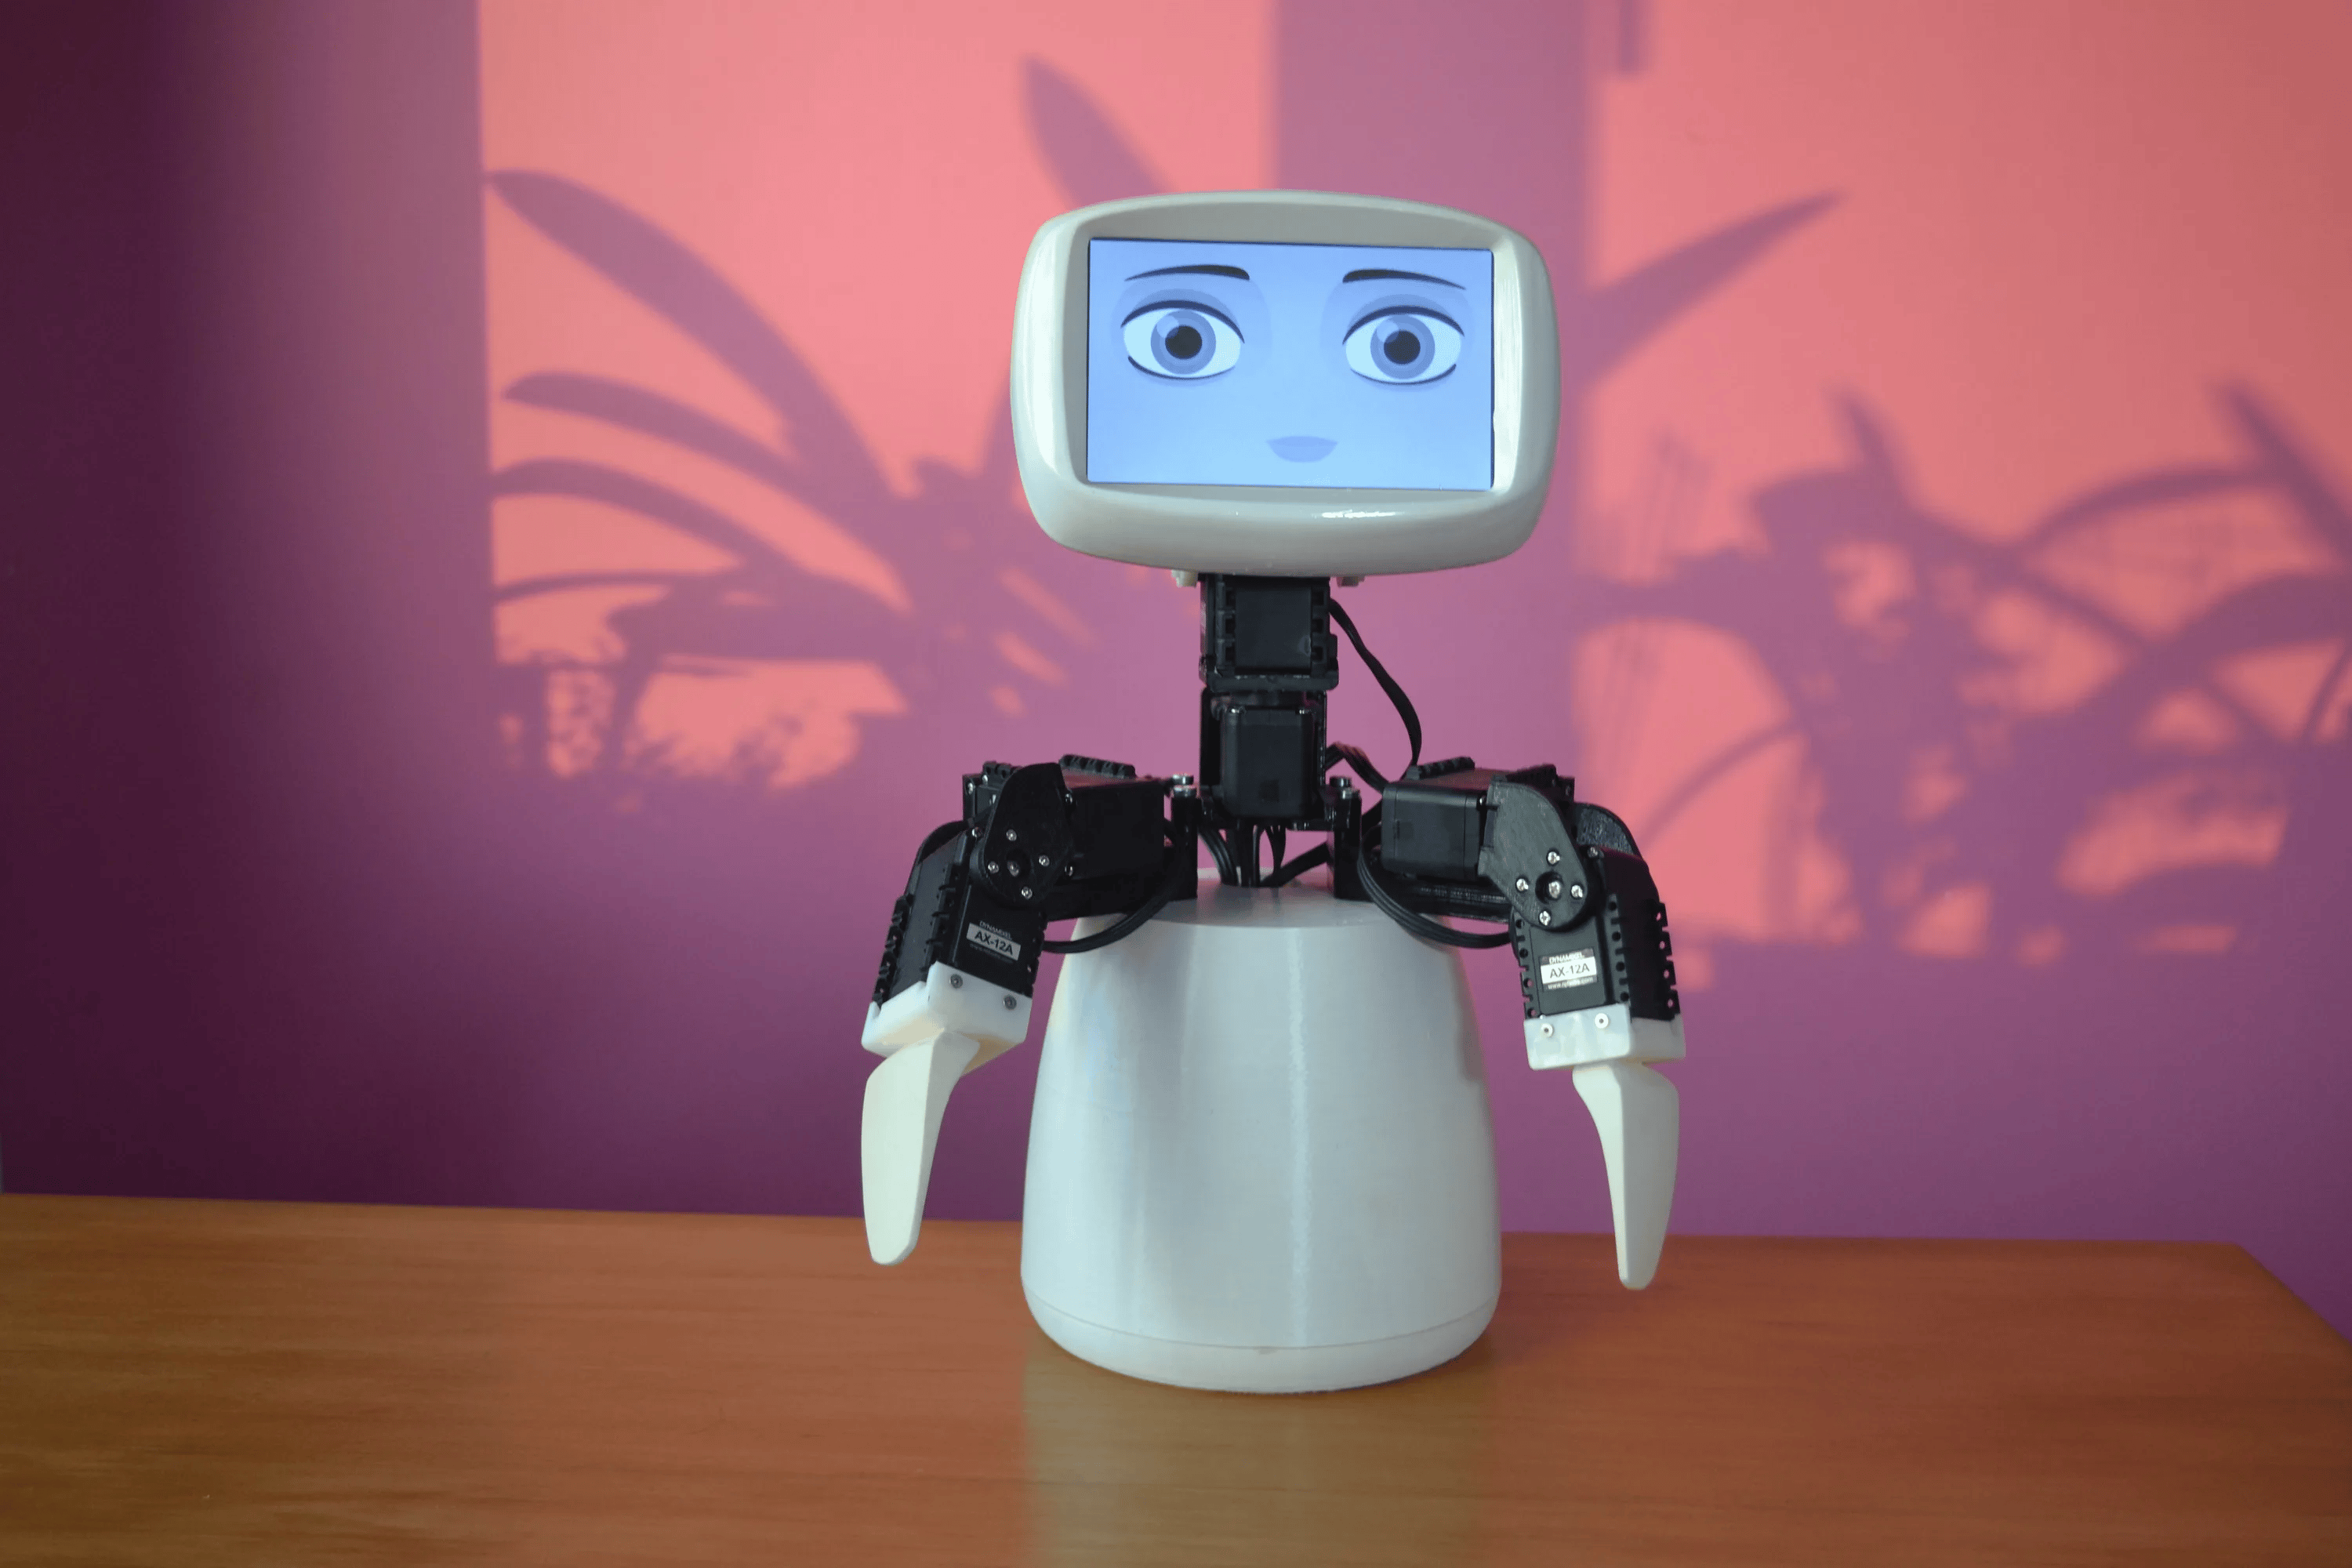
\includegraphics[width=\textwidth]{inc/img/f2robot.png}
        \end{column}
    \end{columns}

    \vspace{0.1cm}
    \begin{itemize}
        \item[---] Персонализация робота-собеседника позволяет повысить естественность ЧМВ и качество восприятия робота.
        \item[---] Перспективной представляется модификация метода ведения диалога роботом Ф-2 на основе учёта персональных черт, назначаемых роботу-собеседнику.
        \item[---] Ограничение работы: развлекательная, образовательная и социальная функциональность робота собеседника.
    \end{itemize}
\end{frame}

%----------------------------------------------------------------------------------------
%    ЦЕЛЬ И ЗАДАЧИ
%----------------------------------------------------------------------------------------

\begin{frame}{\centering Цель и задачи работы}
    \textbf{Цель работы}~---~разработка модифицированного метода ведения диалога роботом Ф-2 с учётом персональных черт робота.

    \vfill
    \textbf{Задачи:}
    \begin{itemize}
        \item[---] провести анализ подходов к описанию персональных черт;
        \item[---] провести обзор существующих решений, в которых применены различные подходы к описанию персональных черт;
        \item[---] провести анализ исходного метода ведения диалога роботом Ф-2;
        \item[---] разработать модифицированный метод ведения диалога роботом Ф-2 с учётом персональных черт робота;
        \item[---] реализовать разработанный метод;
        \item[---] провести оценку качества результатов реализованного метода.
    \end{itemize}
\end{frame}

%----------------------------------------------------------------------------------------
%    ПЕРСОНАЛЬНАЯ ЧЕРТА
%----------------------------------------------------------------------------------------

\begin{frame}
    \frametitle{Персональные черты}
    \small\textbf{Черта}~---~это диспозиция, то есть склонность вести себя определённым образом, проявляющаяся в поведении человека в широком спектре ситуаций. %Черта может быть описана

    \textbf{Грань черты} --- конкретный признак черты.

    \begin{figure}
        \centering
        \includesvg[width=\textwidth,height=0.62\textheight,keepaspectratio,inkscapelatex=false]{BFT}
    \end{figure}
\end{frame}

%%----------------------------------------------------------------------------------------
%%    РОБОТ Ф-2
%%----------------------------------------------------------------------------------------
%
%\begin{frame}
%    \frametitle{Базовый метод ведения диалога роботом Ф-2}
%    \begin{columns}[T]
%        \begin{column}{0.48\textwidth}
%            \textbf{Основные компоненты Ф-2:}
%            \begin{itemize}
%                \item[---] лингвистический;
%                \item[---] сценарный;
%                \item[---] управляющий.
%            \end{itemize}
%            \vspace{0.3cm}
%            Лингвистический компонент строит семантическое представление входного сообщения.
%        \end{column}
%        \begin{column}{0.48\textwidth}
%            \textbf{Выбор реакции:}
%            \begin{itemize}
%                \item[---] сравнение представления с посылками сценариев;
%                \item[---] вычисление весов активированных сценариев;
%                \item[---] выбор сценария с наибольшим весом;
%                \item[---] воспроизведение BML-кадра поведения.
%            \end{itemize}
%        \end{column}
%    \end{columns}
%    \vfill
%    \textbf{Место модификации:} между вычислением весов д-сценариев и выбором сценария для реализации.
%\end{frame}

%----------------------------------------------------------------------------------------
%    ВЫБОР МОДЕЛИ ЛИЧНОСТИ
%----------------------------------------------------------------------------------------

\begin{frame}
    \frametitle{Выбор подхода к описанию персональных черт}
    \begin{center}
        \scriptsize
        \setlength{\tabcolsep}{2pt}
        \renewcommand{\arraystretch}{1.4}
        \begin{tabularx}{\textwidth}{|
            >{\raggedright\arraybackslash}m{0.31\textwidth}|
            >{\centering\arraybackslash}X|
            >{\centering\arraybackslash}X|
            >{\centering\arraybackslash}X|
            >{\columncolor{LightCyan}\centering\arraybackslash}X|
            >{\centering\arraybackslash}X|
        }
                \hline
                \textbf{Критерий} &
                \textbf{Олпорт} &
                \textbf{Айзенк} &
                \textbf{Кеттел} &
                \textbf{БПЧ} &
                \textbf{MBTI} \\
                \hline
                Опубликованы свидетельства о применимости подхода при моделировании поведения персонажей ДС или роботов-собеседников &
                -- & + & -- & + & -- \\
                \hline
                Вариативность моделируемых личностей &
                Высокая & Высокая & Высокая & Высокая & \shortstack{Ограничена\\16 типами} \\
                \hline
                Наличие теста или опросника для определения типа личности исходя из соотношения черт &
                -- & + & + & + & + \\
                \hline
                Композиция (обобщение) других диспозициальных подходов &
                -- & -- & -- & + & -- \\
                \hline
                Кросс-культурная устойчивость &
                \resizebox{0.92\linewidth}{!}{Неустойчива} &
                \resizebox{0.92\linewidth}{!}{Устойчива} &
                \resizebox{0.92\linewidth}{!}{Неустойчива} &
                \resizebox{0.92\linewidth}{!}{Устойчива} &
                \resizebox{0.92\linewidth}{!}{Неустойчива} \\
                \hline
        \end{tabularx}
    \end{center}

    Выбран подход <<Большая пятёрка черт>> (БПЧ)

\end{frame}

%----------------------------------------------------------------------------------------
%    СРАВНЕНИЕ СПОСОБОВ УЧЁТА ПЕРСОНАЛЬНЫХ ЧЕРТ
%----------------------------------------------------------------------------------------

\begin{frame}
    \frametitle{Сравнение способов учёта персональных черт}
    \footnotesize
    Критерии:
    \begin{itemize}
        \item[---] \textbf{K1} --- выбранный подход к описанию персональных черт;
        \item[---] \textbf{K2} --- выбранные черты подхода;
        \item[---] \textbf{K3} --- каналы коммуникации или поведенческие параметры.
    \end{itemize}

    \vspace{0.05cm}
    \begin{center}
        \scriptsize
        \setlength{\tabcolsep}{2pt}
        \renewcommand{\arraystretch}{1.2}
        \begin{tabularx}{\textwidth}{|
            >{\raggedright\arraybackslash}m{0.30\textwidth}|
            >{\centering\arraybackslash}m{0.10\textwidth}|
            >{\centering\arraybackslash}m{0.15\textwidth}|
            >{\raggedright\arraybackslash}X|
        }
                \hline
                \textbf{Решение} & \textbf{K1} & \textbf{K2} & \centering\arraybackslash\textbf{K3} \\
                \hline
                Генератор синтетических личностей &
                БПЧ &
                E, C, A &
                вербальный, паравербальный, невербальный \\
                \hline
                PERSONAGE &
                БПЧ &
                E &
                вербальный \\
                \hline
                Генератор эмоционального состояния &
                БПЧ &
                E, A, N, O &
                невербальный \\
                \hline
                Роботизированная голова KMC-EXPR &
                БПЧ &
                E &
                невербальный \\
                \hline
                Робот-помощник после инсульта &
                Айзенк &
                E &
                вербальный, паравербальный, невербальный \\
                \hline
                \rowcolor{LightCyan}
                Модель на основе нечёткой логики &
                БПЧ &
                все черты &
                пространственные и двигательные параметры \\
                \hline
        \end{tabularx}
    \end{center}

    \vfill
    \scriptsize
    где \(E\) --- экстраверсия, \(A\) --- доброжелательность, \(C\) --- добросовестность, \(N\) --- нейротизм, \(O\) --- открытость опыту.
\end{frame}

%----------------------------------------------------------------------------------------
%    ПРЕДЛАГАЕМЫЙ МЕТОД
%----------------------------------------------------------------------------------------

\begin{frame}
    \frametitle{Модифицированный метод ведения диалога роботом Ф-2}
    \vspace{-0.2cm}
    \noindent\includesvg[width=\textwidth,inkscapelatex=false]{f2_speech_method}

    \vfill
    \begin{minipage}{1\textwidth}
        \raggedright
        \small
        Предлагаемая модификация метода ведения диалога роботом Ф-2 --- введение блока \textbf{A3}: существующие сценарии поведения робота в ответ на входное предложение изменяются с учётом назначаемого роботу профиля

    \end{minipage}
\end{frame}

%----------------------------------------------------------------------------------------
%    ПРИМЕР МОДИФИКАЦИИ РЕАКЦИИ
%----------------------------------------------------------------------------------------


\begin{frame}
    \frametitle{Пример модификации реакции робота \\ предлагаемым методом}
    \begin{figure}
        \centering
        \includesvg[height=0.8\textheight,keepaspectratio,inkscapelatex=false]{example_of_modification}
    \end{figure}
\end{frame}

%----------------------------------------------------------------------------------------
%    ФОРМАЛИЗАЦИЯ
%----------------------------------------------------------------------------------------

\begin{frame}
    \frametitle{Формализация задачи}
    \begin{columns}[T]
        \begin{column}{0.43\textwidth}
            \footnotesize
            Входной набор активированных д-сценариев:
            \[
                A = \{\langle d_i, w_i \rangle \mid i = 1..N\},
            \]
            где \(d_i\) --- активированный д-сценарий, \(w_i\) --- его исходный вес.

            \vspace{0.15cm}
            Модуль вычисляет множитель \(m_i\) и пересчитывает вес:
            \[
                w'_i = clip(w_i \cdot m_i).
            \]

            \vspace{0.15cm}
            Выходной набор:
            \[
                A' = \{\langle d_i, w'_i \rangle \mid i = 1..N\}.
            \]
        \end{column}
        \begin{column}{0.55\textwidth}
            \begin{figure}
                \centering
                \includesvg[width=\textwidth,height=0.72\textheight,keepaspectratio,inkscapelatex=false]{fpz}
            \end{figure}
        \end{column}
    \end{columns}
\end{frame}

%----------------------------------------------------------------------------------------
%    БЛОК A3
%----------------------------------------------------------------------------------------

\begin{frame}
    \frametitle{Блок модификации поведения на основе персональных черт (детализация)}
    \begin{figure}
        \centering
        \includesvg[width=\textwidth,height=0.76\textheight,keepaspectratio,inkscapelatex=false]{filter_method_specified}
    \end{figure}
\end{frame}

%----------------------------------------------------------------------------------------
%    ПАРАМЕТРЫ МЕТОДА
%----------------------------------------------------------------------------------------

\begin{frame}
    \frametitle{Параметры предлагаемого метода}
    \tiny
    \begin{columns}[T,onlytextwidth]
        \begin{column}{0.49\textwidth}
            \scriptsize\textbf{Профиль персональных черт робота}\tiny
            \[
                P = \{\langle p_j, value_j \rangle \mid j = 1..K\},
            \]
            \(p_j\) --- грань личности; \(value_j\) --- терм, описывающий
            способ проявления грани \(p_j\); \(K\) --- число используемых граней.

            \vspace{0.3cm}
            \scriptsize\textbf{Параметры отношения робота к собеседнику}\tiny
            \[
                R = \{\langle r_l, value_l \rangle \mid l = 1..L\},
            \]
            \(r_l\) --- параметр отношения робота к собеседнику;
            \(value_l\) --- значение параметра \(r_l\);
            \(L\) --- количество параметров отношения.
            \[
                value_l \in D^R_l,\quad
                D^R_l = T^R_l \;\textrm{или}\; D^R_l = X^R_l \subseteq \mathbb{R}.
            \]
            Если параметр задаётся числом, дополнительно задаются терм-множество
            \(T^R_l\) и функции принадлежности:
            \[
                \mu^R_{l,t}: X^R_l \rightarrow [0; 1], \quad t \in T^R_l.
            \]
        \end{column}

        \begin{column}{0.49\textwidth}
            \scriptsize\textbf{Параметры ситуации}\tiny
            \[
                S = \{\langle s_h, value_h \rangle \mid h = 1..M\},
            \]
            \(s_h\) --- параметр ситуации, \(value_h\) --- значение данного
            параметра; \(M\) --- количество параметров ситуации.
            \[
                value_h \in D^S_h,\quad
                D^S_h = T^S_h \;\textrm{или}\; D^S_h = X^S_h \subseteq \mathbb{R}.
            \]
            Если параметр задаётся числом, дополнительно задаются терм-множество
            \(T^S_h\) и функции принадлежности:
            \[
                \mu^S_{h,t}: X^S_h \rightarrow [0; 1], \quad t \in T^S_h.
            \]

            \vspace{0.15cm}
            \textbf{Обозначения для областей значений}\\
            \(D^R_l, D^S_h\) --- области значений; \(T^R_l, T^S_h\) ---
            множества допустимых лингвистических значений; \(X^R_l, X^S_h\)
            --- числовые области; \(\mu^R_{l,t}, \mu^S_{h,t}\) ---
            функции принадлежности терму \(t\).

            \vspace{0.15cm}
            Профиль \(P\), отношение к собеседнику \(R\) и ситуация \(S\) имеют
            одинаковую структурную форму: это множества параметров, значения
            которых далее используются в правилах перевзвешивания д-сценариев.
        \end{column}
    \end{columns}
\end{frame}

%----------------------------------------------------------------------------------------
%    НЕЧЕТКИЙ ВЫВОД
%----------------------------------------------------------------------------------------

\begin{frame}
    \frametitle{Вычисление коэффициентов для перевзвешивания}
    \scriptsize
    Правило перевзвешивания в рамках предлагаемого метода имеет вид:
    \[
        IF\; P_r \land C_r \land R_r\; THEN\; d_i \rightarrow e_r,
    \]
    \(P_r\) --- условие по профилю персональных черт, \(C_r\) --- условие по параметру ситуации,
    \(R_r\) --- условие по параметру отношения робота к собеседнику, \(e_r\) --- терм влияния.

    \vspace{0.1cm}
    \textbf{Пример правила:}
    \[
        \begin{aligned}
            &IF\; (\text{Настойчивость} = \text{средняя}) \land
            (\text{Общительность} = \text{низкая}) \land \\
            &(\text{Степень навязчивости} = \text{критичная}) \land
            (\text{Круг общения} = \text{дальний}) \\
            &THEN\; \text{\texttt{ты\_попал\_в\_плохое\_место}} \rightarrow
            \text{сильное усиление}.
        \end{aligned}
    \]
    \vfill
    Используется нечёткий вывод Сугено нулевого порядка.
    \begin{center}
        \begin{tabular}{|l|c|}
            \hline
            \textbf{Терм влияния правила} & \textbf{Множитель} \\
            \hline
            сильное ослабление & 0.50 \\
            \hline
            ослабление & 0.75 \\
            \hline
            без изменения & 1.00 \\
            \hline
            усиление & 1.25 \\
            \hline
            сильное усиление & 1.50 \\
            \hline
        \end{tabular}
    \end{center}
\end{frame}

%----------------------------------------------------------------------------------------
%    АЛГОРИТМ
%----------------------------------------------------------------------------------------

\begin{frame}
    \frametitle{Алгоритм вычисления коэффициентов перевзвешивания активированных д-сценариев}
    \begin{figure}
        \centering
        \includesvg[width=\textwidth,height=0.76\textheight,keepaspectratio,inkscapelatex=false]{scenario_reweighting_algorithm}
    \end{figure}
\end{frame}

%----------------------------------------------------------------------------------------
%    СТРУКТУРА ПО
%----------------------------------------------------------------------------------------

\begin{frame}
    \frametitle{Структура ПО}
    \small
    В качестве языка программирования был выбран Python3.\\
    В качестве среды разработки был использован PyCharm.

    \vspace{0.2cm}
    \begin{figure}
        \centering
        \includesvg[width=\textwidth,height=0.66\textheight,keepaspectratio,inkscapelatex=false]{components_diagram}
    \end{figure}
\end{frame}

%----------------------------------------------------------------------------------------
%    ДИАГРАММА ПОСЛЕДОВАТЕЛЬНОСТИ
%----------------------------------------------------------------------------------------

% надо растянуть по ширине
\begin{frame}
    \frametitle{Диаграмма последовательности}
    \begin{figure}
        \centering
        \includesvg[width=\textwidth,height=0.76\textheight,keepaspectratio,inkscapelatex=false]{diagram}
    \end{figure}
\end{frame}

%%----------------------------------------------------------------------------------------
%%    ИНТЕРФЕЙС
%%----------------------------------------------------------------------------------------
%
%\begin{frame}
%    \frametitle{Графический интерфейс программы}
%    \begin{columns}[T]
%        \begin{column}{0.5\textwidth}
%            \begin{figure}
%                \centering
%                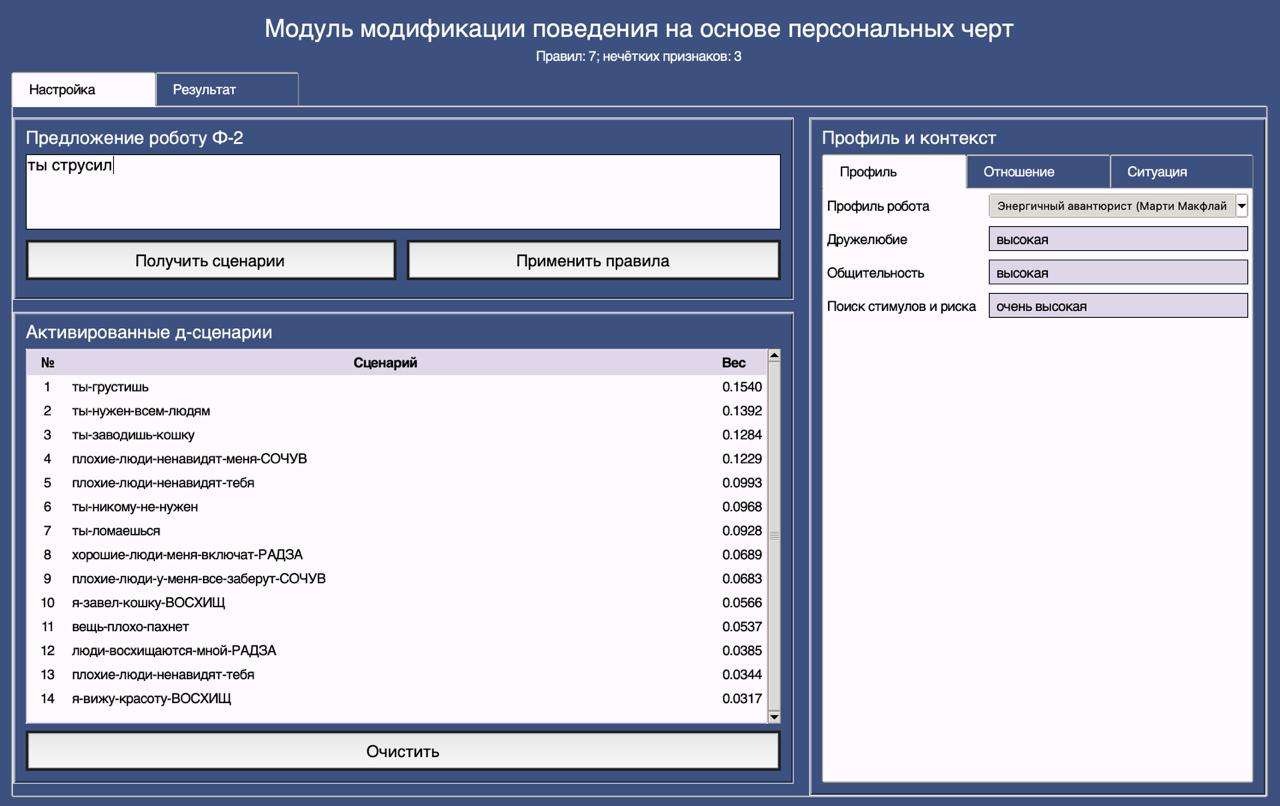
\includegraphics[width=\textwidth]{inc/img/gui_setup.png}
%            \end{figure}
%            \centering
%            \small Вкладка настройки
%        \end{column}
%        \begin{column}{0.5\textwidth}
%            \begin{figure}
%                \centering
%                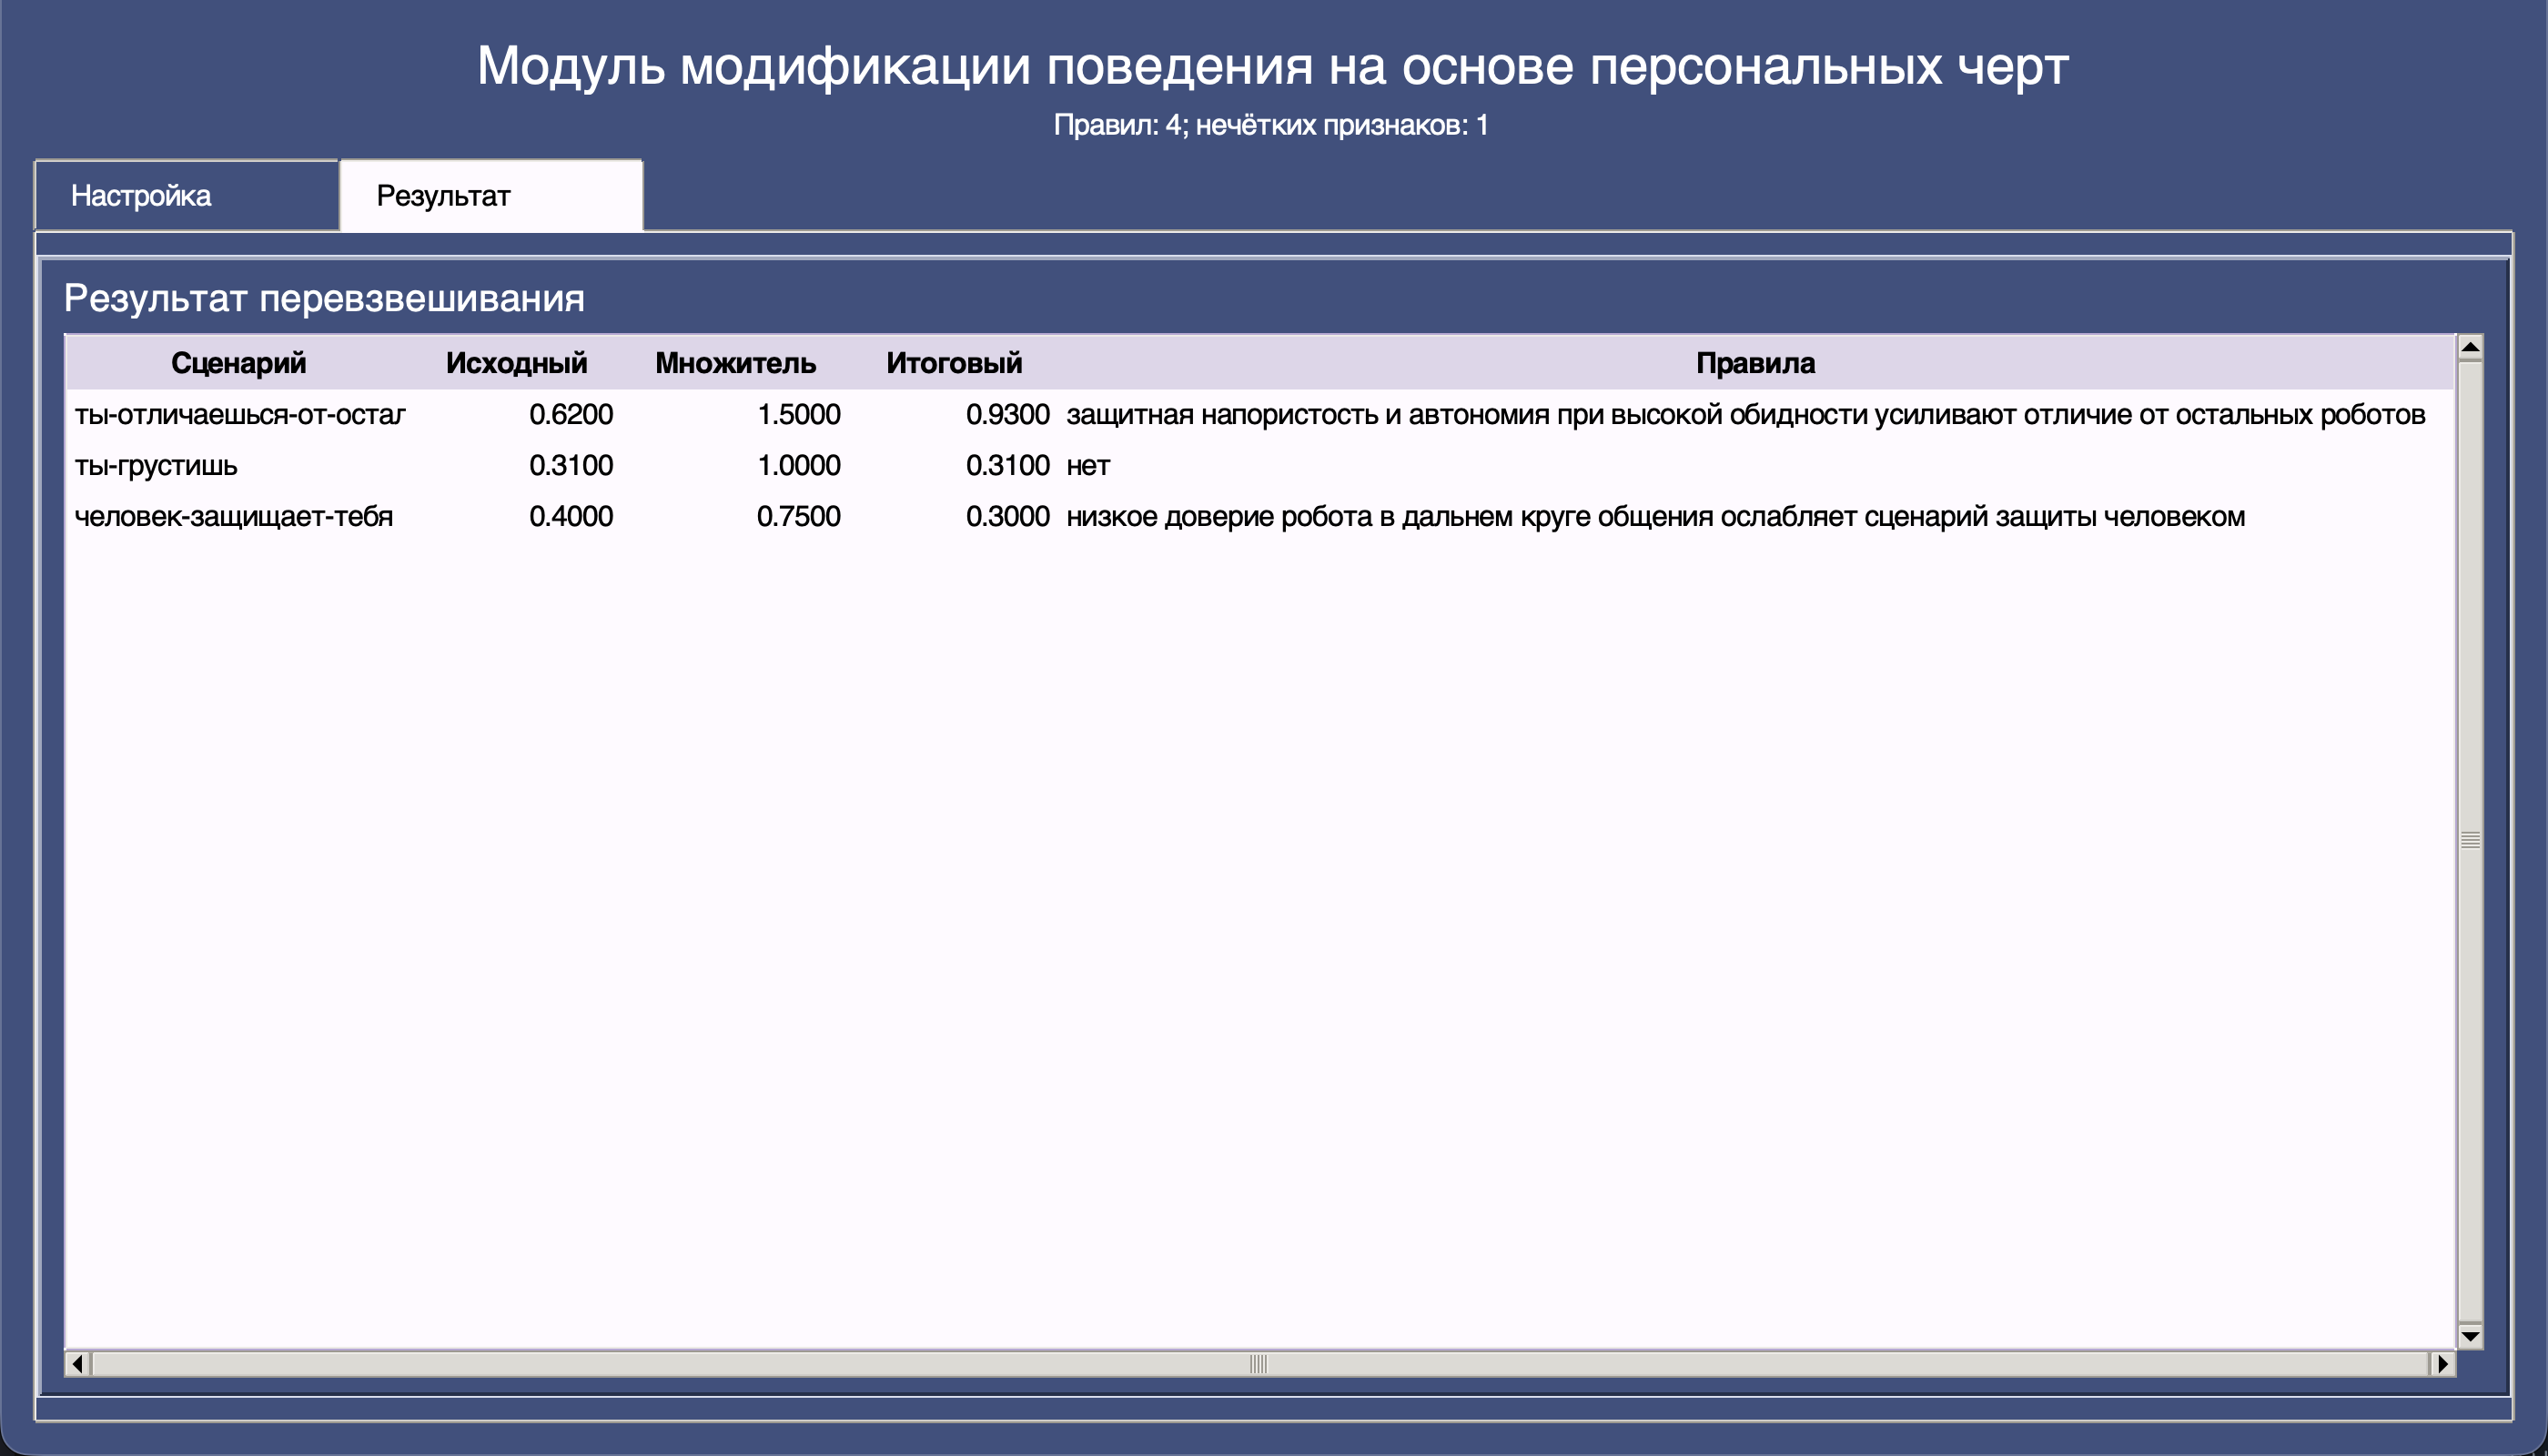
\includegraphics[width=\textwidth]{inc/img/gui_result.png}
%            \end{figure}
%            \centering
%            \small Вкладка результата
%        \end{column}
%    \end{columns}
%    \vfill
%    \small
%    Интерфейс позволяет получить активированные д-сценарии, задать профиль и контекст, применить правила и увидеть исходные веса, множители, итоговые веса и сработавшие правила.
%\end{frame}

%----------------------------------------------------------------------------------------
%    ИССЛЕДОВАНИЕ
%----------------------------------------------------------------------------------------

\begin{frame}
    \frametitle{Отбор реакций для применения в роботах-компаньонах}
    %\textbf{Цель исследования}~---~определить, различают ли респонденты
    %проявления конкретных граней на материале конкретных реакциями робота.

    %\vfill
    \textbf{Условия исследования:}
    \begin{itemize}
        \item[---] 19 респондентов в возрасте от 22 до 37 лет
        \item[---] 30 граней Большой пятёрки черт
        \item[---] 3 степени проявления каждой грани: низкая, средняя, высокая
        \item[---] 90 пар \guillemotleft ситуация + степень\guillemotright{}
    \end{itemize}

    \vfill
    \textbf{Критерий отбора} --- согласованность ответов респондентов: если респонденты соглашаются в выборе реакций, сопоставляя их со степенями проявления граней профиля, это будет свидетельствовать в пользу следующего:
    \begin{itemize}
        \item[---] общее понимание респондентами различий в поведении, обусловленных гранями БПЧ
        \item[---] сценарии реакции с большим числом голосов в заданных условиях следует отбирать для дальнейшего использования при формировании коммуникативных реакций роботом-собеседником, тогда как сценарии с единичными голосами следует отбраковывать или резко понижать их вес среди активированных сценариев
    \end{itemize}
\end{frame}


\begin{frame}
    \frametitle{Исследовательская процедура}
    \begin{itemize}
	\item Этап 1. Для каждой грани описать правила, которые при заданных значениях степени проявления грани БПЧ модифицируют веса активированных сценариев, при этом правило может затрагивать более одного сценария из пула д-сценариев робота Ф-2.
	\item Этап 2. Составить набор ситуаций, в которых будут рассматриваться реакции в коммуникации.
	\item Этап 3. Составить анкету и предложить респондентам оценить предлагаемые реакции.
	\item Этап 4. Агрегировать полученные ответы, оценить согласованность мнений. Выполнить сравнительный анализ полученных мнений, в том числе на предмет применимости первичного набора правил.
	\item Этап 5. Выполнить отбор реакций.
	\item Этап 6. Сформулировать рекомендации о модификации набора правил на основании интерпретации мнений респондентов.
\end{itemize}
\end{frame}

\begin{frame}
    \frametitle{Анкетирование респондентов}
    \begin{columns}[T,onlytextwidth]
        \begin{column}{0.43\textwidth}
            \small
            Для каждой грани:
            \begin{itemize}
                \item[---] Дается описание грани
                \item[---] Затем респонденту предлагается выбрать 1--2 предложения,
                раскрывающих сценарий реакции из представленного набора так,
                чтобы реакция больше всего соответствовала каждой из трех
                степеней проявленности грани.
            \end{itemize}
            В начале анкеты предлагается разбор примера
        \end{column}
        \begin{column}{0.55\textwidth}
            \begin{figure}
                \centering
                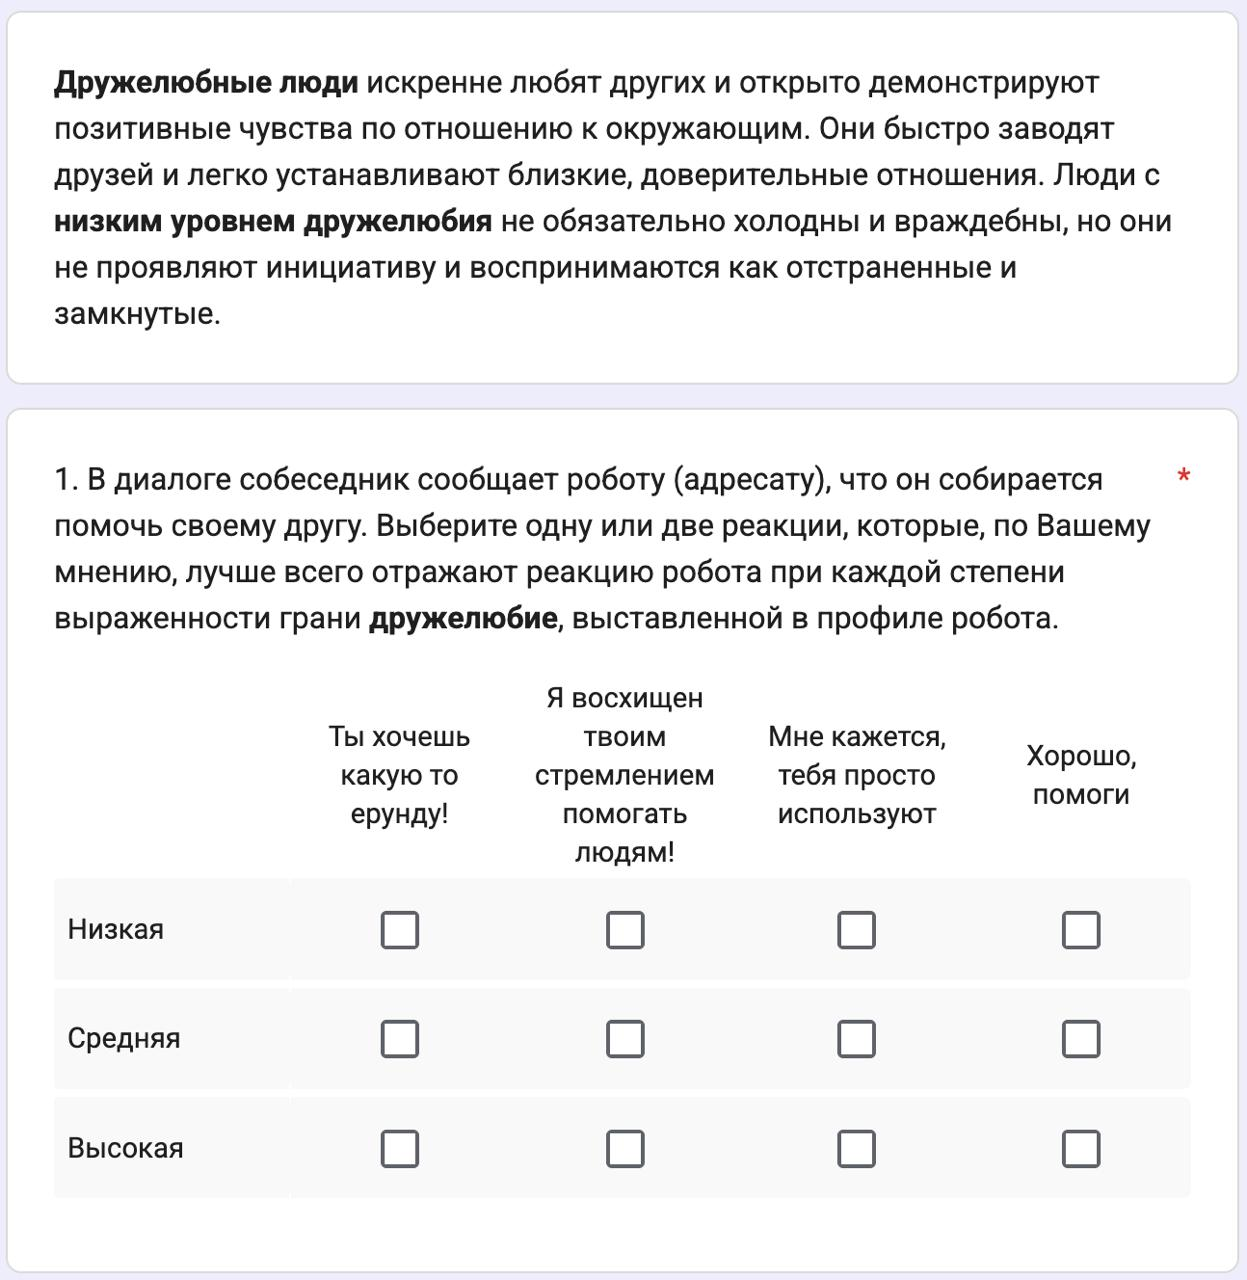
\includegraphics[width=\textwidth,height=0.72\textheight,keepaspectratio]{inc/img/example_of_questionarre_answer.png}
            \end{figure}
        \end{column}
    \end{columns}
\end{frame}

\begin{frame}
    \frametitle{Результаты исследования}
    \begin{columns}[T,onlytextwidth]
        \begin{column}{0.48\textwidth}
            \textbf{Согласованность ответов}
            \vspace{0.15cm}
            \begin{itemize}
                \item[---] средняя согласованность: \textbf{50~\%};
                \item[---] полное совпадение ответов: \textbf{0 из 90} случаев;
                \item[---] согласованность не ниже 75~\%: \textbf{12 из 90} случаев;
                \item[---] согласованность не ниже 67~\%: \textbf{24 из 90} случаев.
            \end{itemize}
        \end{column}
        \begin{column}{0.48\textwidth}
            \textbf{По степеням проявления}
            \vspace{0.15cm}
            \begin{center}
                \renewcommand{\arraystretch}{1.25}
                \begin{tabular}{|l|c|}
                    \hline
                    \textbf{Степень} & \textbf{Согласованность} \\
                    \hline
                    Низкий & 57~\% \\
                    \hline
                    Средний & 41~\% \\
                    \hline
                    Высокий & 53~\% \\
                    \hline
                \end{tabular}
            \end{center}

        \end{column}
    \end{columns}

    \vfill
    Крайние степени проявления в среднем распознавались лучше, чем средние.
\end{frame}

\begin{frame}
    \frametitle{Согласованность ответов по граням}
    \scriptsize
    \begin{columns}[T,onlytextwidth]
        \begin{column}{0.49\textwidth}
            \textbf{Грани с наибольшей согласованностью мнений об обусловленных ими реакциях}
            \vspace{0.08cm}
            \begin{center}
                \renewcommand{\arraystretch}{1.2}
                \begin{tabular}{|p{0.70\linewidth}|c|}
                    \hline
                    \textbf{Грань} & \textbf{Согл.} \\
                    \hline
                    интеллектуальная любознательность & 81~\% \\
                    \hline
                    альтруизм & 79~\% \\
                    \hline
                    самодисциплина & 79~\% \\
                    \hline
                    дружелюбие & 70~\% \\
                    \hline
                    исполнительность & 67~\% \\
                    \hline
                    доверчивость & 63~\% \\
                    \hline
                    осторожность & 63~\% \\
                    \hline
                    воображение & 63~\% \\
                    \hline
                \end{tabular}
            \end{center}
        \end{column}
        \begin{column}{0.49\textwidth}
            \textbf{Грани с наименьшей согласованностью мнений об обусловленных ими реакциях}
            \vspace{0.08cm}
            \begin{center}
                \renewcommand{\arraystretch}{1.2}
                \begin{tabular}{|p{0.70\linewidth}|c|}
                    \hline
                    \textbf{Грань} & \textbf{Согл.} \\
                    \hline
                    моральность & 28~\% \\
                    \hline
                    уязвимость & 28~\% \\
                    \hline
                    подавленность & 30~\% \\
                    \hline
                    самоэффективность & 33~\% \\
                    \hline
                    поиск острых ощущений & 35~\% \\
                    \hline
                    чувствительность к оценке & 35~\% \\
                    \hline
                    настойчивость & 37~\% \\
                    \hline
                    жизнерадостность & 37~\% \\
                    \hline
                \end{tabular}
            \end{center}
        \end{column}
    \end{columns}

    \vfill
    \small
    Грани с согласованностью не менее 75~\% рекомендуется использовать
    в первичной конфигурации правил. \\
    Моральность и уязвимость люди различают хуже всего
\end{frame}

\begin{frame}
    \frametitle{Частота выбора отдельных реакций}
    \vspace{-0.15cm}
    \begin{figure}
        \centering
        \includesvg[width=\textwidth,height=0.52\textheight,keepaspectratio,inkscapelatex=false]{histogram}
    \end{figure}

    \vspace{-0.3cm}
    \scriptsize
    \begin{itemize}
        \item[---] 127 из 389 сочетаний <<вопрос + реакция>> выбраны большинством респондентов: не менее 10 из 19; соответствующие сценарии реакций и обусловливающие их правила рекомендуются к применению в роботе-собеседнике
        \item[---] 155 сочетаний находятся в промежуточной зоне: от 4 до 9 респондентов; соответствующие сценарии реакций и обусловливающие их правила необходимо переработать и оценить повторно
        \item[---] 86 сочетаний выбраны 1-2 респондентами и отбор не прошли
    \end{itemize}

    \vfill
    \small
    Предложенные метод и исследовательская процедура рекомендуются к применению для роботов-компаньонов
\end{frame}


%%----------------------------------------------------------------------------------------
%%    ТЕСТИРОВАНИЕ И РЕЗУЛЬТАТЫ
%%----------------------------------------------------------------------------------------
%
%\begin{frame}
%    \frametitle{Тестирование программной реализации}
%    \begin{itemize}
%        \item[---] Проверена отправка сообщения в API Ф-2.
%        \item[---] Проверено извлечение пар \texttt{scenario}/\texttt{proximity}.
%        \item[---] Проверена загрузка JSON-конфигураций профилей, параметров отношения, параметров ситуации и правил.
%        \item[---] Проверена фаззификация численных признаков и расчёт степеней принадлежности термам.
%        \item[---] Проверена агрегация нескольких правил для одного д-сценария через взвешенное среднее.
%        \item[---] Проверены негативные случаи: пустое предложение, отсутствие адреса API, некорректные профили и правила.
%    \end{itemize}
%    \vfill
%    \textbf{Результат:} все позитивные и негативные функциональные тесты пройдены успешно.
%\end{frame}

%----------------------------------------------------------------------------------------
%    ЗАКЛЮЧЕНИЕ
%----------------------------------------------------------------------------------------

\begin{frame}{\centering Заключение}
    В ходе выполнения работы были решены следующие задачи:
    \begin{itemize}
        \item[---] проведен анализ существующих подходов к описанию персональных
черт;
        \item[---] проведен обзор существующих решений, в которых применены
различные подходы к описанию персональных черт;
        \item[---] проведен анализ исходного метода ведения диалога роботом Ф-2;
        \item[---] разработан модифицированный метод ведения диалога роботом Ф-2 с
учётом персональных черт робота;
        \item[---] реализован разработанный метод;
        \item[---] проведена оценка качества результатов реализованного метода.
    \end{itemize}
    \vfill
    \textbf{Цель работы достигнута:} разработан модифицированный метод ведения диалога роботом Ф-2 с учётом персональных черт робота.

\end{frame}
    \begin{frame}{\centering Демонстрация}

    Ограничение: на вход подаётся простое повествовательное или побудительное предложение на русском языке

    Для демонстрации описаны несколько профилей:

    Защитно-дистанцированный профиль:

    \begin{itemize}
        \item[---] грань \textbf{настойчивость} --- средняя
        \item[---] грань \textbf{сотрудничество} --- низкое
        \item[---] грань \textbf{общительность} --- низкая
        \item[---] грань \textbf{чувствительность к оценке} --- высокая
    \end{itemize}

    Авторитарно-контролирующий:

    \begin{itemize}
        \item[---] грань \textbf{настойчивость} --- высокая
    \end{itemize}

    Профиль --- основа для модификации базового поведения робота, основанного на хотя бы 2 сценариях реакций с наибольшими весами.
\end{frame}

\end{document}
